\documentclass{beamer}
\usepackage[T1]{fontenc}
\usepackage[utf8]{inputenc}
\usepackage{lmodern}
\usepackage[polish]{babel}
\usepackage{graphicx}

\usetheme{AGH}

\title[Dodatkowe aplikacje w aparatach słuchowych]{Dodatkowe aplikacje w aparatach\\słuchowych: wystrzałowe gadżety\\czy przydatne ułatwienia}

\author[B. Bułat, T. Drzewiecki]{Bartłomiej Bułat, Tomasz Drzewiecki}

\date[2011]{23.01.2012}

\institute[AGH]
{Wydział EAIiIB\\ 
Katedra Automatyki i Inżynierii Biomedycznej
}

\setbeamertemplate{itemize item}{$\maltese$}

\begin{document}

{
%\usebackgroundtemplate{
\includegraphics[width=\paperwidth]{titlepage}} % wersja angielska
\usebackgroundtemplate{
\includegraphics[width=\paperwidth]{titlepagepl}} % wersja polska
 \begin{frame}
   \titlepage
 \end{frame}
}

%---------------------------------------------------------------------------


\begin{frame}
\frametitle{Wstęp}

\begin{block}{Aparaty słuchowe}

Ubytek słuchu powoduje duże utrudnienia życiowe. Aparaty słuchowe mają za zadanie wspomóc osoby z wadami słuchu.

\end{block}
\end{frame}

\begin{frame}
\frametitle{Krótka historia I}
Początki aparatów słuchowy sięgają XVII wieku. Wtedy używa trąbek do poprawy odbierania sygnałów dźwiękowych.
\begin{figure}
    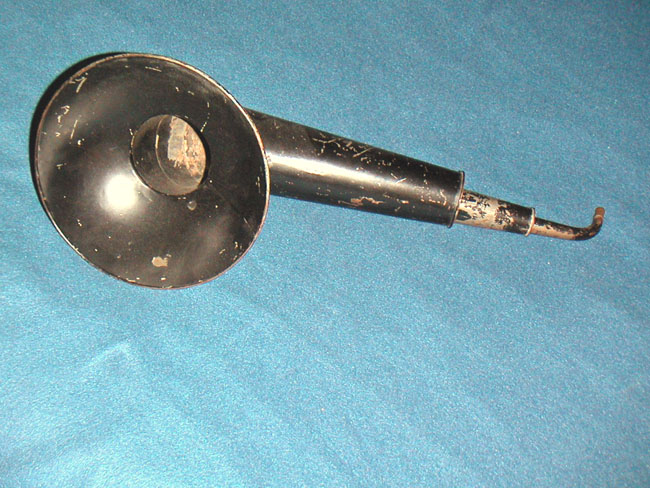
\includegraphics[width=0.25\textwidth]{trumpet}
    \caption{Trąbka słuchowa}
    \label{fig:trumpet}
\end{figure}
\end{frame}

\begin{frame}
\frametitle{Krótka historia II}
Pierwsze urządzenia elektroniczne do poprawy słuchu stworzono w XX wieku. Były one duże oraz ciężkie, więc trudne do noszenia.
\begin{figure}
    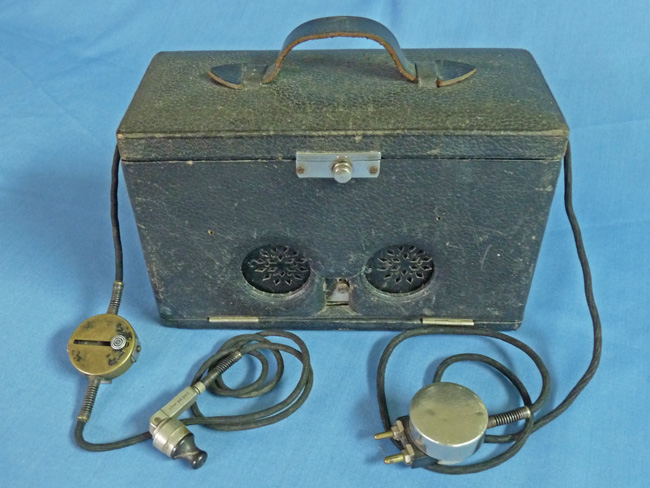
\includegraphics[width=0.3\textwidth]{siemens_old}
    \caption{Siemens/Fortiphone Model M-22 "Booster Flat" Carbon Hearing Aid}
    \label{fig:siemens-old}
\end{figure}
\end{frame}

\begin{frame}
W ciągu całego XX wieku ulepszano i pomniejszano aparaty. W tym momencie na rynku są dostępne aparaty, które łatwo ukryć wśród włosów oraz posiadające funkcje dodatkowe.
\frametitle{Krótka historia III}
\begin{figure}
    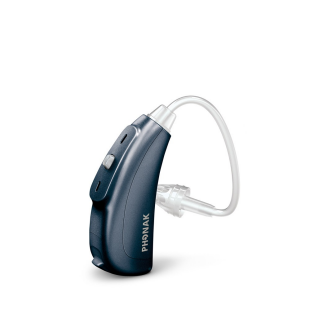
\includegraphics[width=0.25\textwidth]{phonak}
    \caption{Phonak Bolero Q}
    \label{fig:phonak}
\end{figure}
\end{frame}

\begin{frame}
\frametitle{Tłumienie szumu}
Większość obecnie dostępnych na rynku aparatów realizuje funkcję tłumienia szumu. Jest to pożądana funkcja dodatkowa, pozwalająca urządzeniu reagować podobnie jak ludzki słuch, który jest w stanie rejestrować tylko interesujące nas dźwięki. 

Dodatkową opcją, dostępną w mniejszej gamie modeli, jest redukcja szumu powstałego przez wiatr wiejący wokół mikrofonu. To jest również przydatna funkcja pozwalająca na lepsze działanie aparatu nie tylko w pomieszczeniach zamkniętych.
\end{frame}

\begin{frame}
\frametitle{Usuwanie sprzężeń zwrotnych}
Ta funkcja, podobnie jak tłumienie szumu, jest również bardzo pożądana w aparatach słuchowych. Także jest dostępna w większości oferowanych modeli.

Sprzężenia mogą się pojawić podczas normalnej pracy urządzenia i powodować dyskomfort oraz chęć zrezygnowania z aparatu. Dlatego to jest ważny dodatek.
\end{frame}

\begin{frame}
\frametitle{Tryb działania zależny od otoczenia}
Pozwala na zmianę parametrów aparatu w zależności od otoczenia. Zwiększa to komfort używania urządzenia, poprawia możliwości rozumienia słów. Jednak przy użyciu wcześniejszych funkcji nie jest niezbędna. Poprawne i wystarczające zrozumienie słów można osiągnąć bez jej obecności.

Ta funkcja jest dostępna w mniejszej ilości aparatów niż dwie poprzednie.
\end{frame}

\begin{frame}
  \frametitle{Bezprzewodowa łączność}

  Rozwój technologii bezprzewodowych, takich jak bluetooth czy wifi pozwala na
  podłączenie aparatu bezpośrednio do urządzenia nadającego dźwięk: radio,
  komputer, etc. Zaletą jest podwyższona jakość dźwięku, wadą odcięcie od
  odgłosów otoczenia - zagrożenie bezpieczeństwa.
\end{frame}


\begin{frame}
  \frametitle{Fizyczna ochrona aparatów}

  Szczelniejsze i wytrzymalsze obudowy pozwalają na korzystanie w każdych
  warunkach środowiska, wilgotności czy zapylenia. Pozwala to osobom noszącym
  aparat na komfortowe uprawianie sportów lub pracę. Dzięki odporności na
  warunki atmosferyczne, aparat może być noszony zawsze - zwiększenie
  bezpieczeństwa pacjenta. Wytrzymalsze materiały utrudniają mechaniczne
  zniszczenie zniszczenie aparatu.
\end{frame}


\begin{frame}
  \frametitle{Dodatkowe akcesoria}

  Dodatkowe akcesoria ułatwiają użytkownikom aparatów codzienne korzystanie z
  urządzenia. Piloty pozwalają na regulację parametrów bez ściągania aparatu z
  ucha. Adaptery bezprzewodowe pozwalają na komunikację z dowolnym urządzeniem
  nadającym dźwięk. Łączniki do okularów, pozwalają na wygodniejsze noszenie
  oprawek, osobom dotkniętym również wadą wzroku. Dodatkowe lub pojemniejsze
  baterie pozwalają używać aparatu nawet długich podróżach.
\end{frame}


\begin{frame}
  \frametitle{Dwa aparaty}

  Dla osób dotkniętych wadą słuchu w obu uszach, noszących dwa aparaty mogą
  zostać udostępnione dodatkowe funkcje podnoszące jakość, np.
  dźwięk przestrzenny. Dodatkowo, użytkowanie
  dwóch aparatów może być kłopotliwe podczas rozmów przez komórkę. Nowoczesne
  urządzenia potrafią rozpoznać taką sytuację i albo wyciszają aparat z
  drugiego ucha, lub przełączają na dźwięk stereo (w obu aparatach słychać to
  co rejestruje ten z przyłożonym telefonem).
\end{frame}

\begin{frame}
  \frametitle{Wygląd}

  Odkąd miniaturyzacja na to pozwala, aparaty mogą przyjmować dowolne kształty,
  kolory i formy. Cecha praktycznie nieistotna, ma duży wpływ na komfort
  psychiczny i akceptację wady przez pacjenta.

  \begin{figure}
    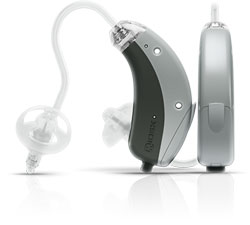
\includegraphics[width=0.3\textwidth]{widex}
    \caption{Widex SUPER}
    \label{fig:widex}
  \end{figure}
\end{frame}

\begin{frame}
  \frametitle{Podsumowanie}
  
  Choć wiele z wymienionych funkcji to przydatne ułatwienia dla
  pacjenta, część z nich to tylko, ogólnie zbędne, gadżety.
\end{frame}

\end{document}

